\chapter{Resultados}
\label{c_resultados}

% Descrever como as crianças interagem com a interface de realidade aumentada
Para simplificar a descrição dos resultados, o \autoref{quadro:equipes} apresenta duplas, trios e indivíduos como equipes que interagiram com a RoPE AR. Houve momentos de troca de participantes, que entraram na brincadeira depois do início ou saíram antes do fim. Nesses casos, a equipe da criança é o grupo no qual ela permaneceu por mais tempo.

\begin{quadro}[!h]
    \caption{Equipes.}
    \label{quadro:equipes}
    \centering
    {
        \begin{footnotesize}
        {\renewcommand{\arraystretch}{1.2}
        \begin{tabular}{|l|l|l|p{11cm}|} 
            \hline
            \textbf{ Equipe/Tempo }                         & \textbf{Criança } & \textbf{Idade} & \textbf{Característica} \\ 
            \hline
            \multirow{2}{*}{Equipe 1. 35min}                & ID1               & 5:10                         & Menino curioso, comunicativo. Discordou de falas do pesquisador e dominou a brincadeira.                           \\ 
            \cline{2-4}
                                                            & ID2               & 5:7                          & Menino menos comunicativo que ID1, mas também falante. Preferiu não disputar o controle da brincadeira.            \\ 
            \hline
            \multirow{2}{*}{Equipe 2. 35min}                & ID3               & 5:10                         & Menina observadora. Preferiu não disputar o controle da brincadeira.                                               \\ 
            \cline{2-4}
            \multicolumn{1}{|c|}{}                          & ID4               & 5:11                         & Menina de personalidade forte. Procurou dominar o acesso ao brinquedo RoPE.                                        \\ 
            \cline{2-4}
            \multicolumn{1}{|c|}{}                          & ID5               & 6:0                          & A mais falante do grupo. Procurou disputar o controle do brinquedo.                                                \\ 
            \hline
            \multirow{2}{*}{Equipe 3. 24min}                & ID6               & 4:10                         & Considerado avançado para a idade. Compreendeu rápido o funcionamento da interface.                                \\ 
            \cline{2-4}
                                                            & ID7               & 3:11                         & Mais novo, ficou impressionado com o fato do brinquedo comer a maçã.                                               \\ 
            \hline
            Equipe 4. 13min                                 & ID8               & 4:3                          & Menino pouco comunicativo, distraído e carinhoso.                                                                  \\ 
            \hline
            \multirow{3}{*}{Equipe 5. 23min}                & ID9               & 4:7                          & Animado, comunicativo e observador.                                                                                \\ 
            \cline{2-4}
                                                            & ID10              & 4:8                          & Considerada de raciocínio rápido.                                                                                  \\ 
            \cline{2-4}
                                                            & ID11              & 4:8                          & Ansioso, animado e curioso. Entrou na metade da brincadeira.                                                       \\ 
            \hline
            \multirow{2}{*}{Equipe 6. 19min}                & ID12              & 4:2                          & Menina mais observadora que comunicativa. Esperava sua vez na brincadeira.                                         \\ 
            \cline{2-4}
                                                            & ID13              & 4:3                          & Menina recém iniciada no CDI. Ansiosa e comunicativa. Tentava pegar o brinquedo na mão.                            \\ 
            \hline
            \multirow{2}{*}{Equipe 7. 10min}                & ID14              & 4:10                         & Menina bastante comunicativa com as demais crianças.                                                               \\ 
            \cline{2-4}
                                                            & ID10              & 4:8                          & Da equipe 5. participou novamente aqui pois ID14 ficou sem dupla.                                                  \\ 
            \hline
            \multirow{2}{*}{Equipe 8. 30min}                & ID15              & 4:7                          & Menino pouco comunicativo, cuidadoso e observador. Precisou de auxílio da professora para entender a brincadeira.  \\ 
            \cline{2-4}
                                                            & ID16              & 4:5                          & Menina observadora. Não quis continuar na brincadeira até o final.                                                 \\ 
            \hline
            \multirow{2}{*}{Equipe 9. 20min}                & ID17              & -                            & Menina falante e brincalhona. Propôs novas trajetórias.                                                            \\ 
            \cline{2-4}
                                                            & ID18              & -                            & Menino agitado e ativo.                                                                                            \\ 
            \hline
            \multirow{2}{*}{Equipe 10. 22min}               & ID19              & -                            & Menino pouco comunicativo, observador. Concentrado nos botões.                                                     \\ 
            \cline{2-4}
                                                            & ID20              & -                            & Menino comunicativo e de respostas criativas.                                                                                    \\
            \hline
            \end{tabular}
        }
        \end{footnotesize}
    }
\end{quadro}

Primeiramente são relatados resultados sobre a análise indutiva. Nessa análise as categorias emergem dos dados. Claramente, m

\section{Análise indutiva}

\subsection{Interação com os blocos}

Seguindo o protocolo, após a ambientação, as crianças passaram a reconhecer os blocos. Era necessário que a criança demonstrasse compreender os símbolos de cada bloco, caso contrário não poderia utilizá-lo para construir algoritmos. De modo geral as crianças apresentaram compreensão do significado de cada bloco, embora sem utilizar um vocabulário padrão. A palavra usada para o bloco Frente foi “cima”, mas enquanto isso a criança apontava para frente. Isso ocorre na fala de ID9 ao apontar para as ferramentas de brinquedo à sua frente (\autoref{quadro:falas_simbolos}). O mesmo ocorreu para os blocos de giro à esquerda e giro à direita: as crianças os trataram ambos como “lado”, porém os seus gestos identificaram a compreensão correta de lateralidade.

\begin{quadro}[htbp]
    \captionquadro{Falas sobre os símbolos dos blocos.}
    \label{quadro:falas_simbolos}
    \begin{footnotesize}
    \begin{longtable}{ | m{.2\textwidth} | m{.7\textwidth} |}
        \hline
        \textbf{Bloco}  & \textbf{Falas e diálogos} \hline
        \endhead
        
        %%%%%%%%%%%%%%%%%%%
    
        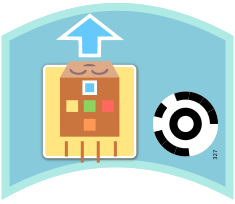
\includegraphics[width=.9\linewidth]{figs/blocks/frente.png} &
    
        \makecell{
            \falapessoa{ID2}{Ele tá botando... o sistema dele pra cima.} \\
            \falapessoa{ID1}{Ele tá olhando pra cima.} \\
            \\
            \falapessoa{ID4}{Rodando} \gesto{Aponta marca fiducial, que é redonda}\\
            \\
            \falapessoa{ID4 e ID5}{Pra aquele (lado)} \gesto{apontam para frente} \\
            \falapessoa{ID3}{Pra aquele} \gesto{aponta pra cima} \\
            \falapessoa{Pesquisador}{Pra cima?} \gesto{ID3 confirma com a cabeça} \\
            \\
            \falapessoa{ID10}{Uma flechinha} \\
            \falapessoa{Pesquisador}{Uma flechinha pra onde?} \\
            \falapessoa{ID10}{Pra cima} \gesto{aponta pra frente} \\
            \falapessoa{ID9}{Tipo daquelas ferramentas} \gesto{aponta brinquedos à frente} \\
            \\
            \falapessoa{Pesquisador}{O que ele tá fazendo aqui nesse desenho?} \\
            \falapessoa{ID13}{Dormindo!} \\
            \\
            \falapessoa{ID17}{Eu acho que ele tá secando as mãos... Eu acho que ele tá indo pra frente} \\
            \\
            \falapessoa{Pesquisador}{Esse bloquinho ele tá indo pra onde?} \\
            \falapessoa{ID15}{Pra pegar a maçã.}
        }

        \\ \hline

        %%%%%%%%%%%%%%%%%%%

        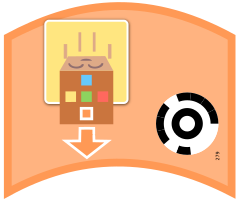
\includegraphics[width=.9\linewidth]{figs/blocks/tras.png} &

        \makecell{
            \falapessoa{ID1}{Esse aqui ele tá olhando pra baixo.} \\
            \\
            \falapessoa{ID10}{Pra baixo.}  \\
            \falapessoa{ID9}{Pra baixo!}  \\
            \falapessoa{Pesquisador}{E onde é pra baixo aqui no robô?} \\
            \falapessoa{ID10}{Grama} \gesto{Aponta para o chão}  \\
            \falapessoa{Pesquisador}{Qual é o botão que faz ele ir pra trás?} \\
            \falapessoa{ID9}{Aqui} \gesto{aponta botão trás} \\
            \\
            \falapessoa{ID17}{Ele tá indo pra trás} \\
            \falapessoa{ID5}{Pra baixo.} \\
            \falapessoa{ID4}{Esse aqui ele tá olhando pra baixo.} \\
        }

        \\ \hline

        %%%%%%%%%%%%%%%%%%%

        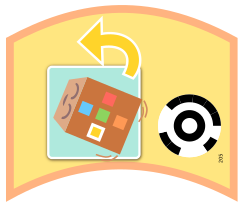
\includegraphics[width=.9\linewidth]{figs/blocks/esquerda.png} &

        \makecell{
            \falapessoa{ID2}{Ele tá olhando pra aquele lado.} \gesto{aponta para a esquerda} \\
            \falapessoa{ID5}{[tá rodando] pra aquele [lado].} \gesto{gira corpo para a esquerda} \\
            \falapessoa{ID10}{Esse aqui ó.} \gesto{aponta para a esquerda}
        }

        \\ \hline

        %%%%%%%%%%%%%%%%%%%

        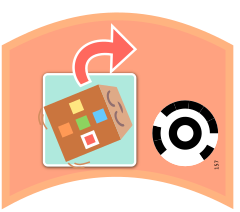
\includegraphics[width=.9\linewidth]{figs/blocks/direita.png} &

        \makecell
        {
            \falapessoa{ID2}{Esse aí ele tá olhando pro lado.} \gesto{aponta para a direita} \\
            \falapessoa{ID10}{Pro lado.} \gesto{aponta para botão do RoPE} \\
            \\
            \falapessoa{Pesquisador}{Ele tá fazendo alguma coisa?} \\
            \falapessoa{ID13}{Tá dormindo! Denovo.} \\
        }

        \\ \hline

        %%%%%%%%%%%%%%%%%%%

        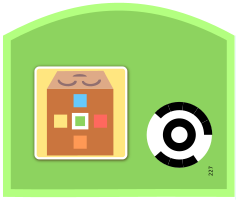
\includegraphics[width=.9\linewidth]{figs/blocks/inicio.png} &

        \makecell{
            \falapessoa{ID1}{Esse aqui também [está olhando pra cima].} \\
            \falapessoa{ID1}{Esse aqui é pra tirar vários.} \\
        }

        \\ \hline

        %%%%%%%%%%%%%%%%%%%

    \end{longtable}
    \end{footnotesize}
\end{quadro}

\begin{quadro}[!h]
   \begin{table_env}
   \caption{Reconhecimento dos blocos}
    \label{quadro:reconhecimentoblocos}
    \begin{tabular}{@{}l m{.6\textwidth} c@{}}
        \toprule
        Categoria                   & Descrição                                                                  & Frequência \\ \midrule
        (fazendo algo) "pro lado"   & Aponta ou fala a direção correta                                           & 5 \\
        (fazendo algo) "pra cima"   & Fala ou aponta direção correta, mesmo falando outras palavras              & 4 \\
        Outros                      & Menciona algo não relacionado a movimento                                  & 3 \\
        (fazendo algo) "pra baixo"  & Aponta ou fala a direção correta usando outras palavras                    & 2 \\
        Relaciona com o botão       & Aponta botão relacionado                                                   & 2 \\
        Menciona esquerda/direita   & Menciona palavras "esquerda" e "direita"\ durante reconhecimento dos blocos & 1 \\
        (fazendo algo) "pra trás"   & Fala a palavra "trás"                                                      & 1 \\
        Rodando                     & Identifica botão frente ou trás como rodando                               & 1 \\
        Aponta pra cima             & Confunde frente com cima, apontando pra cima                               & 1 \\
        Pro chão                    & Diz que o brinquedo está indo pro chão, sem indicar a direção "trás"       & 1 \\ \nidrule
        Indo pegar a maçã           & Diz que o brinquedo está "Indo pegar a maçã"                               & 1 \\ \bottomrule
        \end{tabular}
   \end{table_env}
   \sourceauthor
\end{quadro}

Destaca-se a primeira fala, de ID2, que ao analisar o bloco Frente diz que \fala{ele está botando... o sistema dele pra cima}. Provavelmente a criança não sabe o que é um sistema, mas sabe que é algo associado a um robô. A dinâmica da atividade não permitiu investigar, naquele instante, qual o entendimento da criança sobre o tema, mas temas relacionados à computação apareceram naturalmente em falas posteriores:

\begin{dialogo}
    \gesto{ID2 Clica diversas vezes em todos os botões} \\
    \falapessoa{ID1}{Para, senão ele vai \textbf{bugar}!} \\
    \falapessoa{Pesquisador}{Bugar? o que é bugar?} \\
    \falapessoa{ID1}{É quando ele faz assim ó} \gesto{ID1 e ID2 fazem posição de “estátua”.}
\end{dialogo}

Esta criança, portanto, tem a noção de que \destaque{bugar} é algo a ser evitado e relacionado a travamentos. Outras crianças apresentaram outras justificativas: ID14, como \falapessoa{ID14}{Não anda esse robô. Tava dormindo, coitadinho}. A Equipe 1, além de compreender o significado dos blocos, iniciou a exploração dos mesmos, relacionando-os uns com os outros. As crianças começaram a encaixar os blocos iguais entre si, formando 4 grupos de blocos (4 Frente, 2 Esquerda, 2 Direita, 2 Trás). O pesquisador questionou o motivo de tal agrupamento, conforme o diálogo a seguir:

\begin{dialogo}
    \gesto{Criaças encaixam os blocos)} \\
    \falapessoa{Pesq}{Dá pra montar né? Dá pra encaixar}{01.59} \\
    \gesto{ID2 tenta encaixar peças de cores diferentes)} \\
    \falapessoa{ID1}{Não, esse aqui não pode. Esse aqui não é desse.}{02.06} \\
    \falapessoa{ID2}{É um jogo…}{02.08} \\
    \falapessoa{ID1}{Esse aqui tá olhando pra baixo.}{02.11} \gesto{segura bloco Trás} \\
    \falapessoa{ID1}{Esse aqui vou conectar com esse, e esse conecta com esse}{02.20} \gesto{unindo peças de mesma cor} \\
    \falapessoa{Pesq}{Porque esses assim?}{02.30} \\
    \falapessoa{ID1}{Porque tão olhando pro mesmo lado né!}{02.32} \\
    \falapessoa{Pesq}{Ah... e pela cor né}{02.36} \\
    \falapessoa{ID1}{Não, porque tão olhando pro mesmo lado!}{02.40} \\
    \falapessoa{Pesq}{Ah... entendi...}{02.40}
\end{dialogo}

A justificativa para tal associação, portanto, foi a posição do brinquedo desenhado, e não cor do bloco. Percebendo a similaridade entre pares de blocos, ID1 sugeriu que poderia ser jogado o "Jogo da Memória". O pesquisador e os dois meninos então viraram os blocos com a face para baixo (\autoref{fig:jogo_memoria}), e, cada um a sua vez, virou duas peças. Algo sequer pensado pelo pesquisador foi imaginado pelas crianças.

\begin{figure}[!htbp]
    \begin{center}
    \begin{subfigure}{.5\textwidth}
        \centering
        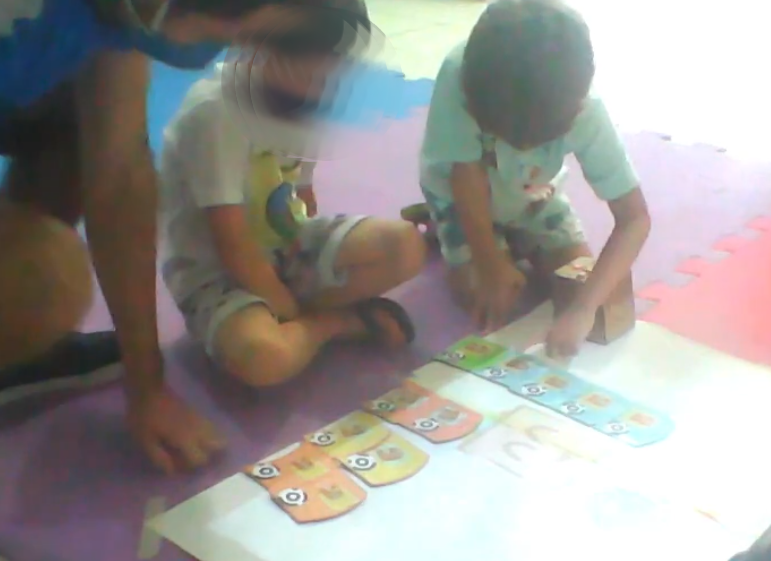
\includegraphics[width=.9\linewidth,fbox]{figs/relacao_blocos.png}
        \caption{Relacionamento entre blocos}
        \label{fig:relacao_blocos}
    \end{subfigure}%
    \begin{subfigure}{.4\textwidth}
        \centering
        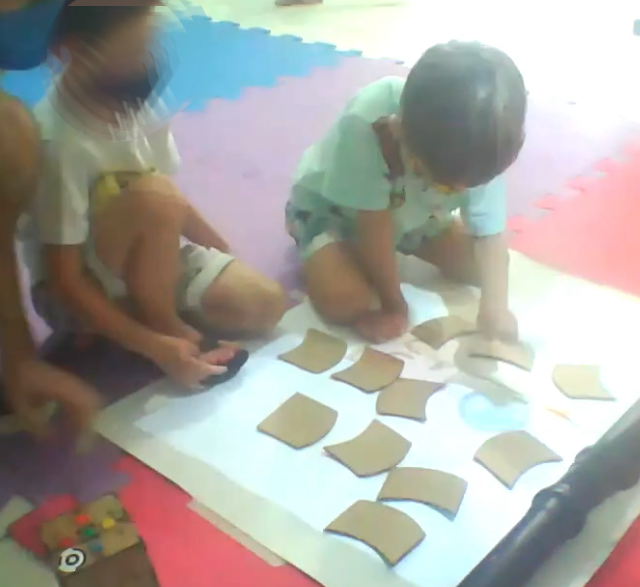
\includegraphics[width=.9\linewidth,fbox]{figs/jogo_memoria.png}
        \caption{Jogo da memória, proposto pela dupla}
        \label{fig:jogo_memoria}
    \end{subfigure}
    \end{center}
    \sourceauthor
    \label{fig:equipe1}
\end{figure}

Algo a ser mencionado é que, durante o jogo da memória, as crianças confundiram os blocos Esquerda e Trás. Isso se deu pela similaridade de cores entre os dois blocos. A criança virou um bloco Trás e um bloco Direita e estava contando como um acerto. ID1, percebendo a diferença, alerta o colega sobre o erro. Esse diálogo revela a interação entre as crianças durante a manipulação dos objetos concretos. 

\begin{dialogo}
    \falapessoa{ID2}{Agora é minha vez.}\gesto{vira peças vermelha e laranja, e acha que acertou}{11.57} \\
    \falapessoa{ID1}{Errou, é diferente.}{12.00} \\ 
    \falapessoa{Pesq}{É diferente né. Mas é parecido, é parecido.}{12.05}
\end{dialogo}

A mesma situação ocorreu com ID8. Ao tentar fazer o brinquedo girar à direita, selecionou o bloco laranja. A Prof\_6 então atua direcionando a atenção da criança para ela perceber o engano. 

\begin{dialogo}
    \falapessoa{Pesq}{Viu que ele foi pra trás, porque aqui tá o bloquinho laranjado. O que ele tem que fazer?} \\
    \falapessoa{ID8}{Vermelho!} \\
    \falapessoa{Pesq}{E qual é o bloquinho vermelho} \\
    \falapessoa{ID8}{Esse aqui ó} \gesto{pega o laranja} \\
    \falapessoa{Prof\_6}{Esse é vermelho, tem certeza? Olha bem.} \\
    \falapessoa{Pesq}{Qual é mais vermelho. Esse ou esse?} \gesto{coloca blocos esquerda e trás lado a lado} \\
    \falapessoa{Prof\_6}{Olha a flechinha se é igual.} \\
    \falapessoa{ID8}{Vermelho é esse.} \gesto{correto} \\
\end{dialogo}

\subsubsection{Associação dos blocos com os botões}

Relação botão blocos

A importância das cores

Percepções de realidade aumentada

Análise dedutiva

% quanto tempo em cada fase?

% quanto tempo em cada estado?


\section{Comparação com os trabalhos relacionados}
\label{sec:comparacao}

\section{Considerações}
\label{sec:}

%Este capítulo pode ter uma última seção como esta denominada ``Considerações'' ou ``Discussão'' consolidando a análise dos resultados.


















































































\begin{comment}

    %A força motriz do design iterativo são as metas do usuário, que são ações que o usuário deseja poder fazer \cite{rogers_design_2013}. Neste trabalho, o alcance das metas de usabilidade se dá quando a criança:
    
    \begin{itemize}
        \item posiciona o brinquedo na posição inicial;
        \item percebe que os blocos representam ações do robô;
        \item sequencia blocos formando um algoritmo;
        \item inicia execução do algoritmo;
        \item altera sequência de blocos; e
        \item percebe blocos destacados durante execução.
    \end{itemize}
    
    Para direcionar a observação, as categorias de análise serão 
    (i) para quais elementos da interface as crianças olham;
    (ii) se e como as crianças manipulam os blocos; 
    (iii) perguntas realizadas; 
    (iv) se e como as crianças comparam os blocos com os símbolos do robô; 
    (v) como ocorre o início da execução; 
    (vi) em que local e direção posicionam o robô; e 
    (vii) se e como os elementos virtuais são percebidos pelas crianças.
    
    %A colaboração será observada quando duas ou mais crianças brincarem em conjunto com os blocos. Esse tipo de evento já foi observado em estudos anteriores \cite{sapounidis_tangible_2019, raabe_estudo_2019}, mas precisa ser confirmado neste estudo para afirmar que a interface apresentada tem os benefícios das interfaces tangíveis. 
    
    % \cite{bardin_alise_1979}.
    \end{comment}